% Elaborado por Jesús Loera, Cesar Valladares y Vrani Chavez

\documentclass[12pt]{article}
\usepackage{blindtext}
\usepackage[T1]{fontenc}
\usepackage[utf8]{inputenc}
\usepackage{amsmath}
\usepackage{amsfonts} 
\usepackage{color}
\usepackage{graphicx}
\usepackage{vmargin}
\usepackage{amssymb}
\usepackage[spanish]{babel}

\usepackage{circuitikz}        %  Dibujar circuitos

\usepackage{mathrsfs,scalerel}  % Laplace
\newsavebox\foobox
\newlength{\foodim}
\newcommand{\slantbox}[2][0]{\mbox{%
        \sbox{\foobox}{#2}%
        \foodim=#1\wd\foobox
        \hskip \wd\foobox
        \hskip -0.5\foodim
        \pdfsave
        \pdfsetmatrix{1 0 #1 1}%
        \llap{\usebox{\foobox}}%
        \pdfrestore
        \hskip 0.5\foodim
}}
\def\Laplace{\ThisStyle{\slantbox[-.45]{$\SavedStyle\mathscr{L}$}}}


\renewcommand{\abstractname}{Descripción}   % Cambiamos el nombre del abstract
\renewcommand{\contentsname}{Contenidos}   % Cambiamos el nombre de contents


\setlength{\jot}{12pt}

\setmargins{2.5cm}       % margen izquierdo
{1.5cm}                        % margen superior
{16.5cm}                      % anchura del texto
{23.42cm}                    % altura del texto
{10pt}                           % altura de los encabezados
{1cm}                           % espacio entre el texto y los encabezados
{0pt}                             % altura del pie de página
{2cm}                           % espacio entre el texto y el pie de página


\renewcommand{\abstractname}{Descripción}   % Cambiamos el nombre del abstract

\makeatletter
\newcommand*{\bigcdot}{}% Check if undefined
\DeclareRobustCommand*{\bigcdot}{%
  \mathbin{\mathpalette\bigcdot@{}}%
}
\newcommand*{\bigcdot@scalefactor}{.5}
\newcommand*{\bigcdot@widthfactor}{1.15}
\newcommand*{\bigcdot@}[2]{%
  % #1: math style
  % #2: unused
  \sbox0{$#1\vcenter{}$}% math axis
  \sbox2{$#1\cdot\m@th$}%
  \hbox to \bigcdot@widthfactor\wd2{%
    \hfil
    \raise\ht0\hbox{%
      \scalebox{\bigcdot@scalefactor}{%
        \lower\ht0\hbox{$#1\bullet\m@th$}%
      }%
    }%
    \hfil
  }%
}
\makeatother

\title{Tarea 1}
\author{Jesus Eduardo Loera Casas 1898887}
\date{\today}

\begin{document}

\begin{titlepage}
    \centering
    {
\includegraphics[width=0.2\textwidth]{FCFM.png}\par}
    \vspace{1cm}
    {\bfseries\LARGE Universidad Autonoma de Nuevo León \par}
    \vspace{1cm}
    {\scshape\Large Facultad de Ciencias Físico Matemáticas \par}
    \vspace{3cm}
    {\scshape\Huge Tarea 2  \par}
    \vspace{3cm}
    {\itshape\Large Ecuaciones de movimiento \par}
    \vfill
    {\Large Autores: \par}
    \vfill
    {\Large Jesús Eduardo Loera Casas 1898887 \par}
    \vfill{\Large Cesar Efrén Valladares Rocha 1841555 \par}
    \vfill
    {\Large Vrani Chavez Islas 1990044 \par}
    \vfill
    {\Large \today \par}
\end{titlepage}

\tableofcontents			% Índice

\begin{center}
    \rule[0mm]{150mm}{0.1mm}		% Para dibujar una linea horizontal de
    % [elevación]{longitud}{grosor}
\end{center}


\begin{abstract}		% ABSTRACT
    
\noindent 				% Anula la sangria de este parrafo
En este documento nuestro equipo presenta el Proyecto 2 del curso de mecánica teórica, 
donde encontramos la ecuación de Euler-Lagrange para una variable independiente y dos dependientes
con ligadura.
\end{abstract}

\begin{center}
    \rule[0mm]{150mm}{0.1mm}
\end{center}

\section{Problema 1}
Encontrar la matriz de transformación que produce un giro de 120 grados a un sistema de 
coordenadas rectangular en torno a un eje fijo (expresar sobre que eje se hace el giro). 
Los ejes coordenados son perpendiculares entre sí.\\

\textbf{Rotación de $\theta = 120^\circ$ alrededor del eje $x_{2}$.}\\
Utilizando cosenos directores para representar la matriz de transformación:

\begin{equation*}
    \lambda_{11} = \cos(x'_{1},x_{1}) = \cos(\theta) \\
    \lambda_{12} = \cos(x'_{1},x_{2}) = \cos\left(\frac{\pi}{2}\right) = 0 \\
    \lambda_{13} = \cos(x'_{1},x_{3}) = \cos\left(\frac{\pi}{2}+\theta\right) = -\sin(\theta) \\
    \lambda_{21} = \cos(x'_{2},x_{1}) = \cos\left(\frac{\pi}{2}\right) = 0 \\
    \lambda_{22} = \cos(x'_{2},x_{2}) = \cos(0) = 1 \\
    \lambda_{23} = \cos(x'_{2},x_{3}) = \cos\left(\frac{\pi}{2}\right) = 0 \\
    \lambda_{31} = \cos(x'_{3},x_{1}) = \cos\left(\frac{\pi}{2}-\theta\right) = \sin(\theta) \\
    \lambda_{32} = \cos(x'_{3},x_{2}) = \cos\left(\frac{\pi}{2}\right) = 0 \\
    \lambda_{33} = \cos(x'_{3},x_{3}) = \cos(\theta) 
\end{equation*}

Entonces la matriz de transformación queda:
\begin{equation*}
    \lambda = \begin{bmatrix}
        \cos(\theta) & 0 & -\sin(\theta) \\
        0 & 1 & 0 \\
        \sen(\theta) & 0 & \cos(\theta)
       \end{bmatrix}
    = \begin{bmatrix}
        \cos(120^\circ) & 0 & -\sen(120^\circ) \\
        0 & 1 & 0 \\
        \sen(120^\circ) & 0 & \cos(120^\circ)
    \end{bmatrix}
\end{equation*}

\begin{equation*}
    \therefore \lambda = \begin{bmatrix}
        -\frac{1}{2} & 0 & -\frac{\sqrt{3}}{2} \\
        0 & 1 & 0 \\
        \frac{\sqrt{3}}{2} & 0 & -\frac{1}{2}
    \end{bmatrix}
\end{equation*}

\section{Problema 2}

\renewcommand{\theenumi}{\alph{enumi}} %Letras minúsculas

% problema a)

\textbf{ a. $ (AB)^{T} = B^{T} A^{T}  $}

\vspace*{0.5 cm}

Consideremos dos matrices cuadradas nxn, A y B:

\begin{equation*}
    A= \begin{bmatrix}
        a_{11} & a_{12} & \cdots & a_{1n} \\
        a_{21} & a_{22} & \cdots & a_{2n} \\
        \vdots & \vdots & \ddots & \vdots \\
        a_{n1} & a_{n2} & \cdots & a_{nn}
    \end{bmatrix}
    B= \begin{bmatrix}
        b_{11} & b_{12} & \cdots & b_{1n} \\
        b_{21} & b_{22} & \cdots & b_{2n} \\
        \vdots & \vdots & \ddots & \vdots \\
        b_{n1} & b_{n2} & \cdots & b_{nn}
    \end{bmatrix}
\end{equation*}

\vspace*{0.15cm}

Utilizemos la siguiente notación:

\begin{gather*}
    A= (a_{ij})_{nxn} \\
    B=(b_{ij})_{nxn}
\end{gather*}

Primero realicemos la multiplicacion de matrices $ \left( AB \right) $:

\begin{align*}
    AB & = (a_{ij})_{nxn} (b_{ij})_{nxn} \\
       & = \left( c_{ij} \right)_{nxn}   \\
\end{align*}

La matriz resultante de dicho producto es la matriz $ \left( c_{ij} \right)_{nxn} $, donde
el término $c_{ij}$ viene dado por la siguiente expresión:

\begin{align*}
    c_{ij} & = \Sigma_{k=1}^{n} a_{ik} b_{kj}
\end{align*}


Ahora, vamos a buscar la transpuesta de la matriz AB:

\vspace*{0.3cm}

Si $(AB)^{T} = \left( c_{ij}^{T} \right)_{nxn} $

\vspace*{0.3cm}

Por defición de matriz transpuesta, el término ij-ésimo $ c_{ij}^{T} $,
de la matriz $(AB)^{T}$ es aquel tal que:

\begin{equation*}
    c_{ij}^{T} = c_{ji}
\end{equation*}

Por lo tanto, tenemos que

\begin{align*}
    c_{ij}^{T} & = c_{ji}                         \\
               & = \Sigma_{k=1}^{n} a_{jk} b_{ki} \\
               & = \Sigma_{k=1}^{n} b_{ki} a_{jk}
\end{align*}

\vspace*{0.3cm}

Prestemos atención en los siguientes $b_{ki}$ y $a_{jk}$.

\vspace*{0.15cm}

El elemento $b_{ki}$, es el mismo que el elemento
tal que $b_{ki}=b_{ik}^{T}$.

\vspace*{0.15cm}

El elemento $a_{jk}$, es el mismo que el elemento
tal que $a_{jk}=a_{kj}^{T}$.

\vspace*{0.15cm}

Por tanto, podemos hacer la siguiente sustitución:

\vspace*{0.3cm}

\begin{align*}
    c_{ij}^{T} & = \Sigma_{k=1}^{n} b_{ki} a_{jk}         \\
               & = \Sigma_{k=1}^{n} b_{ik}^{T} a_{kj}^{T}
\end{align*}

Por defición de multiplicacion de matrices el elemento
$ c_{ij}^{T} = \Sigma_{k=1}^{n} b_{ik}^{T} a_{kj}^{T} $ es el ij-ésimo de la multiplicación de
matrices $ \left(b_{ij}\right)_{nxn}^{T} \left(a_{ij}\right)_{nxn}^{T} $.

\vspace*{0.5cm}

Anteriormente tambíen se mostró que $ c_{ij}^{T}  $ es el ij-ésimo de la multiplicación de
la matriz $(AB)^{T}$.

\vspace*{0.5cm}

$ \therefore $ $(AB)^{T}$ y  $ \left(b_{ij}\right)_{nxn}^{T} \left(a_{ij}\right)_{nxn}^{T} $
son matrices iguales término a término

\begin{equation*}
    \Rightarrow  (AB)^{T} = \left(b_{ij}\right)_{nxn}^{T} \left(a_{ij}\right)_{nxn}^{T}
\end{equation*}

\vspace*{1cm}

% problema b)

\noindent
\textbf{b. $ (AB)^{-1} = B^{-1} A^{-1}  $}

\vspace*{0.5cm}

\noindent
P.D: $ \left(AB\right)^{-1} = B^{-1} A^{-1} $

\vspace*{0.45cm}

\emph{Demostracion.}

\vspace{0.45cm}

Una manera de probar la veracidad de esta igualdad es reducir la expresión a una igualdad
de identidades, así demostramos que la proposición de la que partimos es verdadera.

\vspace{0.2cm}

\begin{gather*}
    \Rightarrow \left(AB\right)^{-1} = B^{-1} A^{-1}
\end{gather*}

\vspace*{0.2cm}

Multiplicamos ambos lados de la igualdad por $AB$ :

\begin{gather*}
    \Rightarrow \left(AB\right)^{-1} \left(AB\right) = B^{-1} A^{-1} \left(AB\right)
\end{gather*}

\vspace*{0.2cm}

Por defición de matriz inversa tenemos que: $ \left(AB\right)^{-1} \left(AB\right) = I $

\begin{gather*}
    \Rightarrow I =B^{-1} A^{-1} \left(AB\right)
\end{gather*}

\vspace*{0.2cm}

Por asociatividad de matrices:

\begin{align*}
    \left(B\right)^{-1} \left(A\right)^{-1} \left(AB\right) & = B^{-1} A^{-1} \left(AB\right) \\
                                                            & =B^{-1} A^{-1} AB               \\
                                                            & =B^{-1} \left(A^{-1} A\right) B
\end{align*}

\vspace*{0.2cm}

Por defición de matriz inversa: $ A^{-1} A = I $

\begin{equation*}
    \Rightarrow I = B^{-1} IB
\end{equation*}

\vspace*{0.2cm}

Como $ IB= B $

\begin{equation*}
    \Rightarrow I = B^{-1} B
\end{equation*}

\vspace*{0.2cm}

Por defición de matriz inversa: $ B^{-1} B = I $

\begin{equation*}
    \Rightarrow I = I
\end{equation*}

\vspace*{0.2cm}

Al reducir la expresión inicial a una igualdad de matrices identidad hemos demostrado la
veracidad de la proposición inicial.

\begin{equation*}
    (AB)^{-1} = B^{-1} A^{-1} \blacksquare
\end{equation*}

\section{Problema 3}
Considere un proyectil que se dispara verticalmente enu un campo gravitatorio constante. Suponiendo que las velocidades
iniciales sean iguales, comparar los tiempos necesarios para que el proyectil alcance su alltura máxima:
\begin{enumerate}
    \item Cuando la fuerza resistente sea nula.
    \item Cuando la fuerza resistente es proporcional a la velocidad instantánea del proyectil.
\end{enumerate}

\noindent \textbf{Modelo matemático:} Sea $y(t)$ la altura de un proyectil en cualquier instante $t$, por la Segunda Ley 
de Newton se tiene:
\begin{align*}
    -mg-mkv &= ma \\
    -g-kv &= a \\
    -g-kv &= \frac{dv}{dt} \\
\end{align*}

\noindent \textbf{Condiciones:} $y(0)=y_{0}$, $\dot{y}(0)=v_{0}$\\
\vspace{5 mm}
\noindent \textbf{Interrogante:} $t_{1}$, tal que el proyectil alcance $y_{1,max}$ con $k=0$; $t_{2}$, tal que el proyectil
alcance $y_{2,max}$ con $k > 0$.

\vspace{5mm}
\textbf{Solución:}
\begin{align*}
    -g-kv &= \frac{dv}{dt} \\
    \frac{dv}{g+kv} &= -dt \\
    \int \frac{dv}{g+kv} &= -\int dt \\
    \frac{\ln(g+kv)}{k} &= -t + C_{1}^{*} \\
    \ln(g+kv) &= -kt + C_{1} \\
    g + kv &= e^{-kt+C_{1}} \\
    g + kv &= e^{C_{1}}e^{-kt} \\
    kv &= C_{1}e^{-kt}-g
\end{align*}

\vspace{5 mm}
Aplicando la condición inicial $v(0)=v_{0}$:
\begin{align*}
    kv_{0} &= C_{1}-g \\
    \Rightarrow C_{1} &= g+kv_{0} \\
    kv &= (g+kv_{0})e^{-kt}-g \\
    \therefore v(t) &= \frac{g+kv_{0}}{k}e^{-kt} - \frac{g}{k}
    %k\frac{dy}{dt} &= (g+kv_{0})e^{-kt}-g \\
    %kdy &= [(g+kv_{0})e^{-kt}-g]dt \\
    %\int kdy &= \int [(g+kv_{0})e^{-kt}-g]dt \\
    %ky &= -\frac{(g+kv_{0})e^{-kt}}{k} - gt + C_{2}^{*} \\
    %y &= -\frac{(g+kv_{0})e^{-kt}}{k^{2}} -\frac{g}{k}t + C_{2} \\
\end{align*}

%\vspace{5 mm}
%Aplicando la condición inicial $y(0)=y_{0}$:
%\begin{align*}
%    y_{0} &= -\frac{g+kv_{0}}{k^{2}} + C_{2} \\
%    \Rightarrow C_{2} &= y_{0} + \frac{g+kv_{0}}{k^{2}} \\
%    y &= -\frac{(g+kv_{0})e^{-kt}}{k^{2}} -\frac{g}{k}t + y_{0} + \frac{g+kv_{0}}{k^{2}} \\
%    \therefore y(t) &= \frac{g+kv_{0}}{k^{2}} (1-e^{-kt}) - \frac{g}{k}t + y_{0}
%\end{align*}

%\vspace{5 mm}
%Se tiene: $kv = C_{1}e^{-kt}-g$. Se busca $t^{*}$, tal que $v(t^{*})=0$.
%\begin{align*}
%    0 &= (g+kv_{0})e^{-kt^{*}}-g \\
%    e^{-kt^{*}} &= \frac{g}{g+kv_{0}} \\
%    -kt^{*} &= \ln \left(\frac{g}{g+kv_{0}}\right) \\
%    \Rightarrow t^{*} &= -\frac{1}{k} \ln \left(\frac{g}{g+kv_{0}}\right)
%\end{align*}

%Sustituyendo $t^{*}$ en $y(t)$:
%\begin{equation*}
%    y(t^{*}) = \frac{g+kv_{0}}{k^{2}} \left(1-\frac{g}{g+kv_{0}}\right) + \frac{g}{k^{2}} \ln \left(\frac{g}{g+kv_{0}} \right) + y_{0}
%\end{equation*}

\vspace{5 mm}
Para hallar el tiempo necesario para que el proyectil alcance $y_{1,max}$ (en un medio con $k>0$), se busca un $t_{1}$ tal que $v(t_{1})=0$.
\begin{align*}
    0 &= (g+kv_{0})e^{-kt_{1}}-g \\
    e^{-kt_{1}} &= \frac{g}{g+kv_{0}} \\
    -kt_{1} &= \ln \left(\frac{g}{g+kv_{0}}\right) \\
    \Rightarrow t_{1} &= -\frac{1}{k} \ln \left(\frac{g}{g+kv_{0}}\right)
\end{align*}

\vspace{5 mm}
En un medio sin resistencia al aire, es decir, con $k=0$, se puede hallar el tiempo para que el proyectil alcance 
$y_{2,max}$ a partir de las ecuaciones básicas de cinemática.
\begin{align*}
    0 &= v_{0} -gt_{2} \\
    v_{0} &= gt_{2} \\
    \Rightarrow t_{2} &= \frac{v_{0}}{g}
\end{align*}

\vspace{5 mm}
A manera de comparación, se obtiene la razón entre el tiempo que le toma al proyectil con resistencia al aire alcanzar
su altura máxima y el tiempo que le toma al proyectil en un medio sisn resistencia. Esto es:
\begin{align*}
    \frac{t_{1}}{t_{2}} &= \frac{-\frac{1}{k} \ln \left(\frac{g}{g+kv_{0}}\right)}{\frac{v_{0}}{g}} \\
    \therefore t_{1} &= \frac{-\frac{1}{k} \ln \left(\frac{g}{g+kv_{0}}\right)}{\frac{v_{0}}{g}} t_{2}
\end{align*}

\section{Problema 4}

Un oscilador armónicose compone de una masa de 100 gramos sujeta a un muelle de constante
recuperadora de 104 dinas/cm. Se desplaza la masa una distancia de 3 cm, soltándose desde 
el reposo. Calcule:

\begin{enumerate}
    \item Frecuencia propia  $ \nu_{o}  $
    \item Periodo  $ \tau_{o}  $
    \item Energía total
    \item Velocidad máxima
\end{enumerate}

\vspace*{0.3 cm}

\begin{figure*}[h]
    \centering
    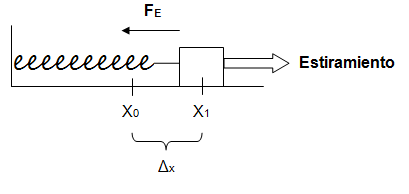
\includegraphics[scale=0.75]{masa_resorte.png}
\end{figure*}

Por la segunda ley de Newton :

\begin{align*}
    F&=ma \\
    -kx&=m \ddot{x} \\
    m \ddot{x}+kx&=0
\end{align*}

Recordemos la frecuencia angular $\omega_{o}^{2}=\frac{k}{m}$, sustituyendo:

\begin{enumerate}
    \item Frecuencia propia  $ \nu_{o}  $
\end{enumerate}

\vspace*{0.35cm}

Recordemos la frecuencia angular $\omega_{o}^{2}=\frac{k}{m}$

\vspace*{0.35cm}

Despejemos la variable $\omega_{o}$

\begin{align*}
    \omega_{o} &= \sqrt{ \frac{k}{m} }
\end{align*}

Recordando la igualdad $ \omega_{o} = 2\pi \nu_{o} $, de donde despejamos
la frecuencia propia $\nu_{o}$

\begin{align*}
    \nu_{o} &= \frac{\omega_{o}}{2\pi}
\end{align*}

Sustituyendo $\omega_{o} = \sqrt{ \frac{k}{m} }$ en la ecuación anterior.

\begin{align*}
    \nu_{o} &= \frac{ \left( \sqrt{ \frac{k}{m} } \right) }{2\pi} \\
    \nu_{o} &= \frac{ 1 }{2\pi} \sqrt{ \frac{k}{m} }
\end{align*}

Sustituyendo en la ecuación anterior:

\begin{align*}
    \nu_{o} &= \frac{ 1 }{2\pi} \sqrt{\frac{( 10^{4} dinas/cm )}{(100 g)}}\\
    \nu_{o} &= 1.6 \frac{1}{s}
\end{align*}

$\therefore$ La frecuencia propia es  $ \nu_{o} = 1.6 \frac{1}{s}$

\vspace*{0.4cm}

b. Periodo  $ \tau_{o}  $

Anteriormente llegamos a la ecuación

\begin{equation*}
    \nu_{o} = \frac{ 1 }{2\pi} \sqrt{ \frac{k}{m} }
\end{equation*}

Recordemos que $\nu_{o}=\frac{1}{\tau_{o}} $, vamos a realizar esta sustitución en la ecuación
anterior:

\begin{align*}
    \frac{1}{\tau_{o}} &= \frac{ 1 }{2\pi} \sqrt{ \frac{k}{m} } \\
                       &= \frac{ \sqrt{k} }{ 2\pi \sqrt{m} }
\end{align*}

Despejamos para el periodo $\tau_{o}$:

\begin{align*}
    \tau_{o}    &= \frac{ 1 }{2\pi} \sqrt{ \frac{k}{m} } \\
                &= \frac{ 2\pi \sqrt{m}  }{ \sqrt{k} } \\
                &= 2\pi \sqrt{ \frac{m}{k} }
\end{align*}

Sustituyendo en la ecuación anterior:

\begin{align*}
    \tau_{o}&= 2\pi \sqrt{ \frac{( 100 g )}{( 10^{4} dinas/cm )} }\\
    \nu_{o} &= 0.62 s
\end{align*}

$\therefore$ El periodo es  $ \tau_{o} = 0.63 $ s

c. Energía total

\vspace*{0.5cm}

Como la energía total es la suma de la energía potencial y la energía cinética, primero
buscaremos expresiones para la velocidad y la posición.

Recordemos la ecuación diferencial del sistema

\begin{equation*}
    m \ddot{x}+kx=0
\end{equation*}

Observación: $ m \ddot{x}+kx=0 $ es una ecuación diferencial lineal
homogénea de orden dos con coeficientes constantes.

\vspace*{0.35cm}

Y de la redacción del problema identificamos las siguientes condiciones iniciales:

\begin{align*}
    x(0) = x_{o} = 3cm \\
    \dot{x} (0) = 0
\end{align*}

Observación: Tenemos condiciones iniciales en $t=0$ por tanto podemos
usar la transformada de Laplace para resolver la ecuación diferencial.

\begin{align*}
    \Laplace \left\{ m \ddot{x}+kx \right\} &= \Laplace \left\{ 0 \right\}
\end{align*}

Recordemos que $ \Laplace \left\{ 0 \right\} = 0 $

\begin{align*}
    \Laplace \left\{ m \ddot{x} \right\} + \Laplace \left\{ kx \right\} &= 0 \\
    m \Laplace \left\{ \ddot{x} \right\} + k \Laplace \left\{x  \right\} &= 0
\end{align*}

Sea $\Laplace \{ x(t) \} = X(s)$ y recordando que $ x(0)= x_{o} = 3cm $ y $ = \dot{x} (0)=0$ 

\begin{itemize}
    \item En $m \Laplace \left\{ \ddot{x} \right\} $: 
\end{itemize}

\begin{align*}
    m \Laplace \left\{ \ddot{x} \right\} &= m \left( s^{2}X(s) -sx(0) - \dot{x}(0) \right) \\
                                         &= m \left( s^{2}X(s) -sx_{o} - 0 \right) \\
                                         &= m s^{2}X(s) -msx_{o}
\end{align*}

\begin{itemize}
    \item En $ k \Laplace \left\{ x \right\} $: 
\end{itemize}

\begin{align*}
    k \Laplace \left\{ x \right\} &= k X(s)
\end{align*}

Sustituyemos las anteriores igualdades en la ecuación diferencial:

\begin{align*}
    m s^{2}X(s) -msx_{o} + k X(s) = 0 
\end{align*}

Ahora despejamos para $X(s)$ :

\begin{align*}
    m s^{2}X(s) -msx_{o} + k X(s) = 0 \\
    m s^{2}X(s) + k X(s) = mx_{o}s 
\end{align*}

\begin{align*}
    X(s) \left( m s^{2} + k \right) &= mx_{o}s \\
    X(s)  &= \frac{mx_{o}s}{m s^{2}+k} \\
    X(s)  &= \frac{mx_{o}s}{ m \left( s^{2} + \frac{k}{m} \right) } \\
    X(s)  &= \frac{x_{o}s}{  s^{2} + \frac{k}{m}  }
\end{align*}

Ahora aplicamos la transformada inversa de Laplace en ambos lados de la ecuación:

%   \Laplace^{-1} \{  \}

\begin{align*}
    \Laplace^{-1} \{ X(s) \} &= \Laplace^{-1} \left\{\frac{x_{o}s}{  s^{2} + \frac{k}{m}} \right\} \\
                             &= x_{o} \Laplace^{1} \left\{\frac{s}{ s^{2} + \frac{k}{m} }\right\} 
\end{align*}

Como  $ \Laplace^{-1} \left\{\frac{s}{s^{2}+k^{2}}\right\} = Cos(kt) $

\vspace*{0.4cm}

\begin{equation*}
    \Rightarrow \Laplace \left\{ \frac{s}{ s^{2} + \frac{k}{m}  } \right\} = Cos \left( \sqrt{ \frac{k}{m} } t \right)
\end{equation*}

\vspace*{0.4cm}

Tambien sabemos que $ \Laplace^{-1} \left\{X(s)\right\} = x(t) $

\vspace*{0.35cm}

Hacemos las sustituciones de las transformadas inversas de Laplace:

\begin{equation*}
    \therefore x(t) = x_{o} Cos \left( \sqrt{ \frac{k}{m} } t \right)
\end{equation*}

Ahora para determinar $\dot{x} (t)$ derivamos a $q(t)$ :

\begin{align*}
    x(t) &= x_{o} Cos \left( \sqrt{ \frac{k}{m} } t \right) \\
    \therefore \dot{x}(t) &= - \sqrt{ \frac{k}{m} } x_{o} Sen \left(  \sqrt{ \frac{k}{m} } t \right)
\end{align*}

Recordando que $T=\frac{1}{2} m \dot{x}^{2}$

\begin{equation*}
    T=\frac{1}{2} m \frac{k}{m} x_{o}^{2} Sen^{2} \left(  \sqrt{ \frac{k}{m} } t \right)
\end{equation*}

Recordando que $V=\frac{1}{2} kx^{2}$

\begin{equation*}
    T=\frac{1}{2} k x_{o} Cos \left( \sqrt{ \frac{k}{m} } t \right)
\end{equation*}

Y como la energía mecánica está dada por $E=T+V$

\begin{align*}
    E   &=T+V \\
        &=\frac{1}{2} m \frac{k}{m} x_{o}^{2} Sen^{2} \left(  \sqrt{ \frac{k}{m} } t \right) 
           + \frac{1}{2} k x_{o}^{2} Cos^{2} \left( \sqrt{ \frac{k}{m} } t \right)
\end{align*}

En ese sistema solo actúan fuerzas conservativas, por tanto la energía se conserva.

Evaluemos la energía en el tiempo $t=0$ :

\begin{align*}
    E(0)&=\frac{1}{2} (100 g) \frac{( 10^{4} dinas/cm )}{m} (3cm)^{2} Sen^{2} \left(  \sqrt{ \frac{( 10^{4} dinas/cm )}{(100 g)} } (0s) \right) \\
        &\hspace{0.23cm}+ \frac{1}{2} ( 10^{4} dinas/cm ) (3cm)^{2} Cos^{2} \left( \sqrt{ \frac{( 10^{4} dinas/cm )}{(100 g)} } (0s) \right) \\
        &= \frac{1}{2} ( 10^{4} dinas/cm ) (3cm)^{2} \\
        &= 45000 ergios
\end{align*}

$\therefore$ La energía total del sistema es de 45000 ergios


d. Velocidad máxima

Retomemos la ecuación de la velocidad que encontramos:

\begin{equation*}
    \dot{x}(t) = - \sqrt{ \frac{k}{m} } x_{o} Sen \left(  \sqrt{ \frac{k}{m} } t \right)
\end{equation*}

Expresemos el módulo de la velocidad:

\begin{align*}
    \left\lVert \dot{x}(t) \right\rVert &= \sqrt{ \left( - \sqrt{ \frac{k}{m} } x_{o} Sen \left(  \sqrt{ \frac{k}{m} } t \right) \right)^{2} } \\
    \left\lVert \dot{x}(t) \right\rVert &= \sqrt{ \frac{k}{m} } x_{o} Sen \left(  \sqrt{ \frac{k}{m} } t \right)
\end{align*}

Esta expresión alcanza su máximo cuando: $ Sen \left(  \sqrt{ \frac{k}{m} } t \right) = 1 $

\begin{equation*}
    \left\lVert \dot{x}(t) \right\rVert_{max} = \sqrt{ \frac{k}{m} } x_{o}
\end{equation*}

Sustituyendo en la ecuación anterior:

\begin{align*}
    \left\lVert \dot{x}(t) \right\rVert_{max} &= \sqrt{ \frac{( 10^{4} dinas/cm )}{(100 g)} } (3cm) \\
                                              &= 30 \frac{cm}{s}  
\end{align*}

$\therefore$ La velocidad máxima es de 30 $\frac{cm}{s}$

\vspace*{0.5cm}

\textbf{Por lo tanto:}

\begin{enumerate}
    \item \textbf{La frecuencia propia es  $ \nu_{o} = 1.6 $ $\frac{1}{s}$}
    \item \textbf{El periodo es  $ \tau_{o} = 0.63 $ s}
    \item \textbf{La energía total del sistema es de 45000 ergios}
    \item \textbf{La velocidad máxima es de 30 $\frac{cm}{s}$}
\end{enumerate}

\end{document}